\section{Benchmark}

The goal of the conducted benchmarking presented in detail in the experimental evaluation is three-fold. First, we want to measure the descriptiveness of the feature descriptors for matching purposes. This is crucial for the recovery of a tracker upon loss of tracking due to occlusion, changed lighting conditions, and alike. Second, we measure the tracking accuracy by integrating each feature descriptor in our 2D tracker and compute the overlap measure using the estimated object position. Third, we profile each separate step required in tracking by detection (key-point detection, descriptor computation and feature matching) in order to evaluate the performance of the feature descriptors for real-time applications.

\subsection{Dataset}

\begin{figure*}[t]
	\vspace{2mm}
\centerline{%
	\subfigure{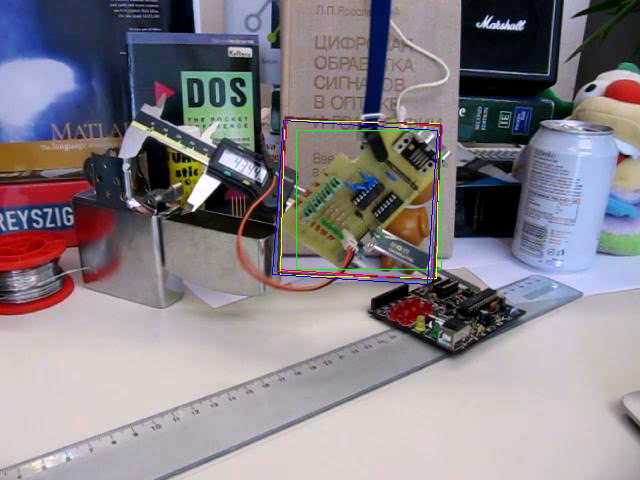
\includegraphics[width=0.19\linewidth]{imgs/dataset/d1.png}}
	\subfigure{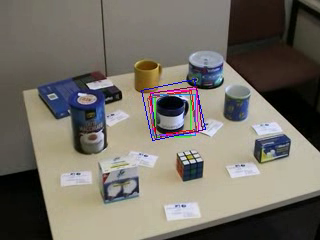
\includegraphics[width=0.19\linewidth]{imgs/dataset/d2.png}}
	\subfigure{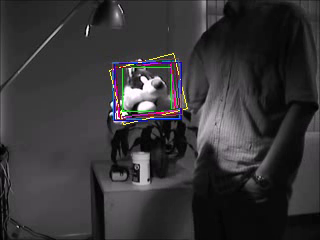
\includegraphics[width=0.19\linewidth]{imgs/dataset/d3.png}}
	\subfigure{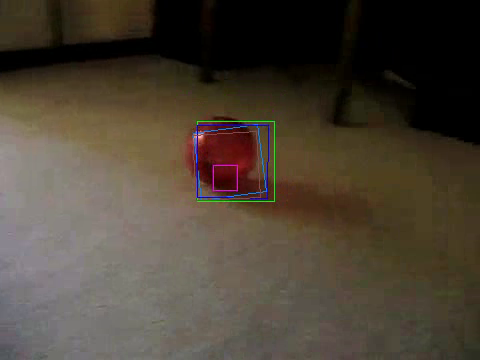
\includegraphics[width=0.19\linewidth]{imgs/dataset/d4.png}}
	\subfigure{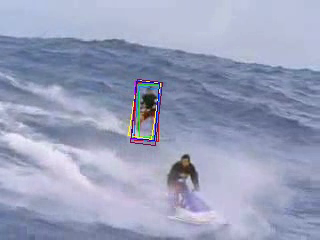
\includegraphics[width=0.19\linewidth]{imgs/dataset/d5.png}}}
	\vspace{-2mm}
\centerline{%
	\subfigure{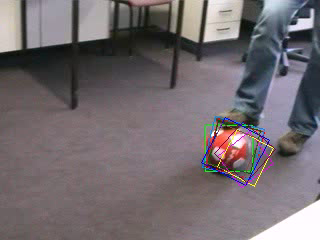
\includegraphics[width=0.19\linewidth]{imgs/dataset/d6.png}}
	\subfigure{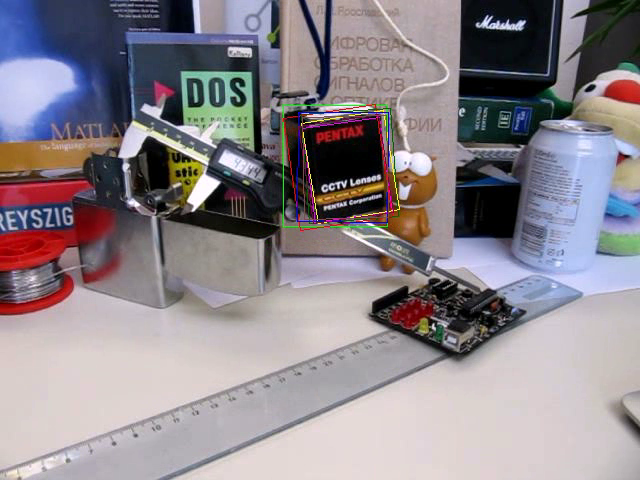
\includegraphics[width=0.19\linewidth]{imgs/dataset/d7.png}}
	\subfigure{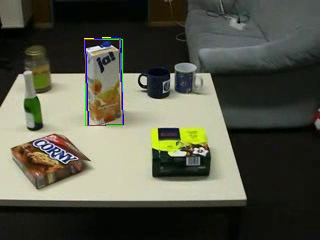
\includegraphics[width=0.19\linewidth]{imgs/dataset/d8.png}}
	\subfigure{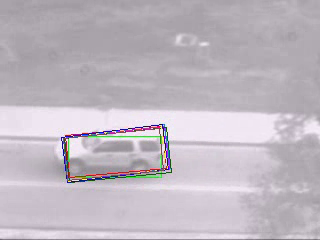
\includegraphics[width=0.19\linewidth]{imgs/dataset/d9.png}}
	\subfigure{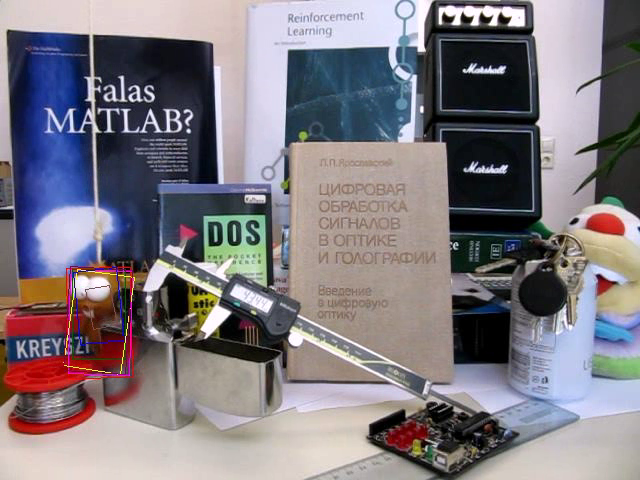
\includegraphics[width=0.19\linewidth]{imgs/dataset/d10.png}}}
\caption{A few example images from the videos used in the benchmark. The sequences include both indoor and outdoor scenes, subjected to changing lightning conditions, 
occlusion, and significant changes in object appearance.}
\vspace{-3mm}
\label{fig:tracking_results}
\end{figure*}


There are several publicly available datasets designed for tracking. However, there is no agreement in the community of the standard structure to store the data. For this reason and in order to facilitate the evaluation, we collected the videos from the different datasets and standardized how these are stored. Each video is stored as a sequence of images while the ground truth, represented by an oriented bounding box of the tracked object, is saved in a separate file where each row corresponds to an image frame defined by the 8 values representing the pairs (x,y) of each vertex of the frame. The generated dataset will be released publicly, along with all the code to perform the experiments and run the evaluation.

\subsection{Matching Evaluation Criteria}
Given a sequence of images $I_{1},...,I_{n}$ with corresponding ground truth bounding boxes $B^g_{1},...,B^g_{n}$ around a target object, we extract a set of key-points $K_1$ from the first image of the sequence and regard all key-points within $B^g_{1}$ as descriptors of the object. For each subsequent image, key-points $K_{t}$ are similarly extracted and then matched to those in the initial set $K_{1}$, generating a list of matches $M_t = \left\lbrace (i,j); ~p_{1,i} \in K_1, p_{t,j} \in K_t \right\rbrace$. Given the bounding boxes a key-point $p_{t,j}$, with a match $(i,j)\in M_t$, is then labeled as follows:
\begin{equation}
%K_{t}^{j} = 
\begin{cases}
\text{true positive},&  \text{ if } p_{t,j} \in B^g_{t} \land p_{1,i} \in B^g_{1} \\
\text{false positive},&  \text{ if } p_{t,j} \notin B^g_{t} \land p_{1,i} \in B^g_{1} \\
\text{false negative},&  \text{ if } p_{t,j} \in B^g_{t} \land p_{1,i} \notin B^g_{1} \\
\end{cases}
\end{equation}

%Given as sequence of images $I_{1},...,I_{n}$ and the bounding box ground truth $gb_{1},...,gb_{n}$, we extract the set of target key-points descriptors $K_{1}$ from the first image of the sequence and label all the key-points within $gb_{1}$ as descriptors of the object. In all subsequent images, key-points $K_{t}$ are extracted and matched with $K_{1}$, generating a list of matches $M_k = \left\lbrace (i,j); i \in K_k, j \in K_1 \right\rbrace$, where \textit{i} indicates a key-point descriptor of our target set $K_{1}$, and \textit{j} a descriptor of our test set. The test set is then labeled as follows:

%\begin{equation}
%K_{t}^{j} = 
%\begin{cases}
%\text{true positive}  \text{ if } K_{t}^{j} \in gb_{n} \land K_{1}^{i} \in gb_{1} \\
%\text{false positive}  \text{ if } K_{t}^{j} \notin gb_{n} \land K_{1}^{i} \in gb_{1} \\
%\text{false negative}  \text{ if } K_{t}^{j} \in gb_{n} \land K_{1}^{i} \notin gb_{1} \\
%\end{cases}
%\end{equation}
%where the pair \textit{i,j} is determined by the matching result $M(i,j)_{k}$. Fig.~\ref{fig:matching} shows an example of how the key-points are labeled. 

\begin{figure}[!htb]
	%\vspace{-2mm}
	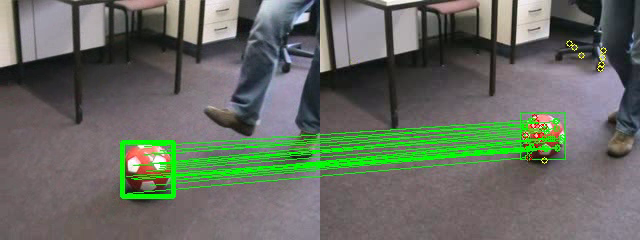
\includegraphics[width=0.95\linewidth]{imgs/matching.png}
\vspace{-2.5mm}	
\caption{Example showing how the matching precision is calculated. The image to the right shows the initial frame of the sequence. Matches in green are true positives. Circles in red are false positives. Yellow circles are false negatives, feature descriptors that are inside the object in the current frame but have a match with the background in our model.}
\label{fig:matching}
\end{figure}

The average ratio of true positives assesses the ability of a tracker to detect the object and potentially recover after the loss of tracking. False negatives are those feature descriptors that appear in the current frame but have no corresponding match to the initial test set $K_{1}$. This may commonly happen when there is a drastic change in appearance of the object. The ratio of false positives is very important to consider since it indicates the average number of outliers that will be used to estimate the pose of the object, resulting in a bad pose estimation if no additional filtering techniques are employed. A widely used filtering technique is to discard all matched key-points if the ratio between the score of the best match and the second best match is below a certain threshold $\rho$. We define a key-point as ambiguous if this criteria is not met. The  number of ambiguous true and false positives is then calculated to evaluate the distinctiveness of the descriptors and evaluate the influence of this common filtering technique on the results.

\subsection{Evaluating tracking precision}
\label{sec:accuracy}

We employ a sparse key-point based tracker to measure the precision of the feature descriptors for tracking. The tracker is initialised using a bounding box in the initial image of a tracking sequence. Inside the bounding box, feature descriptors are extracted and represent the \textit{model} of the tracked object. The algorithm estimates the position of the object, represented as an oriented bounding box, with a combination of sparse optical flow and feature matching as outlined in Algorithm \ref{alg:algorithm}. For the complete details please refer to \cite{pieropan15}.

\begin{algorithm}[!htb]
 \KwData{$I_{1},...,I_{n},B_{1}$}
 \KwResult{$B_{2},...,B_{n}$}
 $K_{1} \gets$ \textbf{extract\_points}($I_{1},B_1$)\;
 \For{$i \gets 2 : n$}{
   $K_{i}^{*} \gets$ track\_points($K_{i-1},I_{i-1},I_i$)\;
   $B_i \gets$ estimate\_pose($K_{i}^{*}$)\;
   $K_{i}' \gets$ \textbf{extract\_points}($I_{i},B_i$)\;
   $M \gets$ \textbf{match\_points}($K_{1},K_{i}'$)\;
   $K_{i} \gets$ merge\_keypoints($K_i^* ,  M$)\;
 }
 \caption{\label{alg:algorithm}Overview of the tracking algorithm used to compute the tracking precision. The feature descriptors are employed in the steps written in bold. }
\end{algorithm}

Our original tracking algorithm used ORB (Oriented Fast and Rotated Brief) proposed by Rublee et al.~\cite{rublee11}. 
We extended the tracking algorithm making it more modular so that tracking can be performed with 
various feature descriptors that we evaluate. To estimate the tracking precision, we used the widely accepted overlap measure:
\begin{equation}
	\Theta (B_{t}, B^g_t) = \frac{B_{t} \cap B^g_t}{B_{t} \cup B^g_t}
\end{equation}
where \textit{$B_{t}$} is the bounding box estimated by our tracker and
\textit{$B^g_t$} is the bounding box provided by the ground truth. We define 
three precision requirements $\Upsilon \in \{0.25, 0.5, 0.75\}$ that indicate low, medium and high tracking accuracy. This is a more indicative evaluation compared to the overall accuracy. For instance, an overall value of 0.5 is ambiguous because it may indicate either a stable average accuracy around the value or a very precise evaluation in part of the video while poor in the rest.
%
%The estimated object box \textit{$B_{t}$} is considered a true positive (TP) for a defined threshold of
%accuracy $\Upsilon$ if:
%
%\begin{equation}
%\begin{cases}
%B_{t} = TP  \text{ if } \Theta(B_{t}, B^g_t) > \Upsilon \\
%B_{t} = FP  \text{ otherwise }\\
%\end{cases}
%\end{equation}
%
%The overall accuracy of the tracker for each precision requirement is calculated as:
%
%\begin{equation}
%\text{recall } = \frac{TP}{\text{TP } + \text{ FN}}
%\end{equation}
%
The overall accuracy of the tracker is then computed for each precision requirement $\Upsilon$ as the fraction of all generated bounding boxes for which $\Theta(B_{t}, B^g_t) > \Upsilon$.


%\missingfigure[figwidth=0.98\linewidth]{Figure showing the estimated bounding boxes and the ground truth to show the different behavior of trackers}

\subsection{Parameter setting}

All the employed descriptors require many parameters to be initialised and run properly. In order to achieve the most fair comparison between them, we decided to keep the values suggested in the original publication of the feature descriptor or the implementation if such was available. However, there are some parameters that most of the feature descriptors share and that we set to the same value. Thus, the maximum number of features extracted is set to 2500 and the number of scale space octaves is set to 4.



